% ============================================================================
%  Loss-Surface Geometry Across the Grokking Transition
%  ICML 2025 Mechanistic Interpretability Workshop
%
%  Drop the body (\maketitle … \bibliography) into the official
%  workshop template (icml2025.sty or neurips_2024.sty).
%  The \documentclass below compiles standalone with the NeurIPS style.
% ============================================================================

\documentclass[12pt]{article}

% ── Submission: replace the two lines below with \usepackage[final]{icml2025} ──
% \usepackage[final]{neurips_2024}
\usepackage[margin=1in]{geometry}
% ──────────────────────────────────────────────────────────────────────────────

\usepackage{natbib}
\usepackage{amsmath,amssymb}
\usepackage{graphicx}
\usepackage{booktabs}
\usepackage{microtype}
\usepackage{hyperref}
\usepackage{xcolor}
\usepackage[capitalize,noabbrev]{cleveref}

\hypersetup{colorlinks=true,
            linkcolor=blue!60!black,
            citecolor=green!50!black,
            urlcolor=blue!60!black}

% ---------------------------------------------------------------------------
\title{%
  Loss-Surface Geometry Across the Grokking Transition:\\
  Two Distinct Notions of Complexity in Competing Loss Basins%
}

\author{%
  Sultan Hassan\\
  \textit{[Institution]}\\
  \texttt{sultanier@gmail.com}
}

\begin{document}
\maketitle

% ===========================================================================
\begin{abstract}
Grokking—the delayed onset of generalisation long after memorisation—provides
a controlled testbed for studying how loss-landscape geometry changes at a
phase transition.  We apply Singular Learning Theory (SLT) to characterise
the competing solutions through the SGLD-estimated Local Learning Coefficient
(LLC), the Hessian trace $\operatorname{tr}(H)$, the largest Hessian
eigenvalue $\lambda_{\max}$, and a new \emph{Fourier bridge} analysis that
tracks circuit-level frequency emergence alongside geometric measures.  Our
central finding is a $110\times$ dissociation between two complexity
estimators post-grokking: $\operatorname{tr}(H)$ drops $24\times$ and
$\lambda_{\max}$ drops $7\times$—confirming that the Fourier solution
occupies a dramatically flatter basin—while the SGLD-LLC stays constant
($\approx\!2{,}000$).  We resolve this contradiction by distinguishing two
levels of degeneracy: (1)~\emph{local flatness}, captured by the
Hessian-estimated LLC~$\hat\lambda_H = \operatorname{tr}(H)/(2\lambda_{\max})
\approx 18$ post-grokking, matching the Fourier circuit's $\sim\!10$--$12$
active frequencies $\times\,2$ parameters; and (2)~\emph{global
multiplicity}, the large number of equivalent Fourier solutions, probed by
the miscalibrated SGLD chain.  The two measures converge quantitatively with
a direct Fourier-amplitude analysis: $\sim\!12$ active frequencies emerge in
the token-embedding spectrum exactly when $\hat\lambda_H$ stabilises,
providing a task-agnostic SLT signal that agrees with mechanistic
interpretability without requiring circuit identification.
\end{abstract}

% ===========================================================================
\section{Introduction}
\label{sec:intro}

Grokking~\citep{power2022grokking} is a striking instance of delayed
generalisation: a transformer trained on modular arithmetic ($a+b \bmod p$)
memorises its training set by step~$500$, then—after a plateau lasting
over $1{,}000$ additional steps—suddenly generalises by step~$2{,}600$.
Mechanistic interpretability has shown that this transition is an algorithmic
switch from a dense attention-based lookup table to a sparse Discrete Fourier
Transform (DFT) circuit that uses only $\sim\!10$ active
frequencies~\citep{nanda2023progress}.

Singular Learning Theory (SLT)~\citep{watanabe2009algebraic} offers a
complementary \emph{geometric} perspective.  Its central quantity—the Real
Log Canonical Threshold (RLCT)—measures how degenerate (flat, high-symmetry)
a loss minimum is.  Lower RLCT implies a broader Bayesian posterior and a
smaller free energy.  SLT therefore predicts that weight decay drives the
model toward the more singular Fourier minimum~\citep{hoogland2024developmental}.
The Local Learning Coefficient (LLC) estimates the RLCT empirically via
SGLD~\citep{lau2023quantifying} and has been used as a continuous phase-
transition detector.

\paragraph{The puzzle.}
When we simultaneously measure the SGLD-LLC and the Hessian geometry across
the grokking arc, we find a stark tension.  The Hessian confirms SLT's
prediction: $\operatorname{tr}(H)$ drops $24\times$ and $\lambda_{\max}$ drops
$7\times$ post-grokking.  But the SGLD-LLC does \emph{not} drop—it remains
$\approx\!2{,}000$ before and after grokking.  This $110\times$ disagreement
between two estimators of the same quantity cannot be dismissed as noise.

\paragraph{Contributions.}
\begin{enumerate}
\item We identify a \textbf{two-level degeneracy structure} at grokking: local
  flatness (Hessian collapses at the transition) and global multiplicity
  (SGLD stays constant), and explain mechanistically why they decouple
  (\S\ref{sec:discussion}).
\item We introduce a \textbf{Fourier bridge}: a direct comparison showing that
  $\sim\!12$ Fourier frequencies emerge in the embedding spectrum at grokking
  onset—exactly when the Hessian-LLC converges to $\hat\lambda_H \approx 18$
  ($\approx\!10$--$12$ freq $\times$ $2$ params)—providing
  a \emph{quantitative link} between mech-interp circuits and SLT geometry
  (\S\ref{sec:results}).
\item We show the \textbf{Hessian-estimated LLC} $\hat\lambda_H$ is a
  task-agnostic, calibration-free proxy for the local RLCT that tracks SLT's
  prediction correctly where SGLD fails (\S\ref{sec:results}).
\item We introduce the \textbf{geometric phase portrait} in
  $(\operatorname{tr}(H),\,\text{LLC})$ space as a new diagnostic that cleanly
  separates memorisation and generalisation basins where the LLC alone cannot
  (\S\ref{sec:results}).
\end{enumerate}

% ===========================================================================
\section{Background}
\label{sec:background}

\paragraph{Singular Learning Theory and the LLC.}
In SLT the RLCT $\lambda$ controls the free energy:
$nF_n(w^*) = nL_n(w^*) + \lambda\log n + O(\log\log n)$
~\citep{watanabe2013widely}.  Smaller $\lambda$ means a more singular
(flatter, more symmetric) minimum with lower free energy—SLT's rigorous
account of implicit regularisation.  The LLC $\hat\lambda$ is estimated via
localised SGLD~\citep{lau2023quantifying}:
\begin{equation}
  \hat\lambda \;=\; \beta n\,\mathbb{E}_{\mathrm{SGLD}}\!\bigl[L(w) -
  L(w^*)\bigr], \qquad \beta = 1/\!\log n,
  \label{eq:llc}
\end{equation}
with a spring $\frac{\gamma}{2}\|w-w^*\|^2$ localising the chain near $w^*$.

\paragraph{Hessian geometry.}
The Hessian $H_{ij} = \partial^2 L / \partial w_i \partial w_j$ encodes the
second-order loss geometry.  Under the Gaussian approximation,
$\lambda \approx \operatorname{rank}(H)/2$, motivating the
\emph{Hessian-estimated LLC}:
\begin{equation}
  \hat\lambda_H \;=\; \frac{\operatorname{tr}(H)}{2\,\lambda_{\max}}.
  \label{eq:h-llc}
\end{equation}
We estimate $\operatorname{tr}(H)$ via the Hutchinson finite-difference
estimator~\citep{hutchinson1990stochastic} and $\lambda_{\max}$ via power
iteration.  Unlike the SGLD estimator, $\hat\lambda_H$ requires no
step-size calibration.

\paragraph{Flatness and generalisation.}
Flat minima generalise better in practice~\citep{keskar2017large}, though the
relationship is subtle~\citep{dinh2017sharp}.  SLT provides the
theoretically grounded account: it is algebraic flatness (the RLCT), not
raw Hessian curvature, that determines Bayesian model
complexity~\citep{watanabe2009algebraic}.

% ===========================================================================
\section{Experimental Setup}
\label{sec:setup}

\paragraph{Task and model.}
We train a one-layer transformer ($d_\mathrm{model}=128$, $4$~heads, $223{,}872$
parameters) to predict $(a+b) \bmod 97$ for $a,b \in \{0,\ldots,96\}$—the
canonical grokking benchmark~\citep{power2022grokking} whose post-grokking
algorithm is fully characterised~\citep{nanda2023progress}.  We use a $30\%$
training split ($2{,}821$ pairs), AdamW~\citep{kingma2015adam,loshchilov2019decoupled}
($\eta=10^{-3}$, weight decay $1.0$), for $5{,}000$ steps.  Weight decay is
essential: it shrinks the high-norm memorisation circuit faster than the
sparse Fourier circuit, providing the energy differential that drives the
transition~\citep{varma2023explaining}.

\paragraph{Measurements.}
At every $250$ steps ($21$ checkpoints) we compute:
\textbf{(i)}~SGLD-LLC via \cref{eq:llc} ($200$ SGLD steps,
$\varepsilon=3\!\times\!10^{-5}$, $\gamma=100$);
\textbf{(ii)}~$\operatorname{tr}(H)$ via $20$ Hutchinson probes with
$\delta=10^{-3}$;
\textbf{(iii)}~$\lambda_{\max}$ via $20$ power-iteration steps;
\textbf{(iv)}~per-layer $\operatorname{tr}(H)$ via block-diagonal Hutchinson
across five component groups (token embedding, attention, FFN, layer-norm,
unembedding); and
\textbf{(v)}~Fourier frequency amplitudes of the token-embedding matrix $W_E$,
defined as the $\ell_2$ power at each frequency $k$:
$A_k = \bigl(\sum_d |\hat{W}_{k,d}|^2\bigr)^{1/2}/p$,
where $\hat{W}_{k,d}$ is the DFT of $W_E[:,d]$ along the token axis.
All Hessian methods use only forward or first-order passes
(\texttt{create\_graph=False}), making them fully MPS/CUDA-safe.

% ===========================================================================
\section{Results}
\label{sec:results}

\paragraph{Training arc.}
\Cref{fig:training} shows the characteristic three-phase grokking arc: fast
memorisation (steps $0$--$500$, train accuracy $\to 100\%$, test
accuracy~$\approx\!28\%$), a memorisation plateau ($500$--$1{,}900$~steps),
and a sharp grokking transition ($1{,}900$--$2{,}600$~steps) after which test
accuracy reaches $100\%$.  Notably, test \emph{loss} rises above the
random-chance baseline ($\log 97 \approx 4.57$) during the plateau—the
lookup-table circuit actively suppresses generalisation.

\begin{figure}[t]
  \centering
  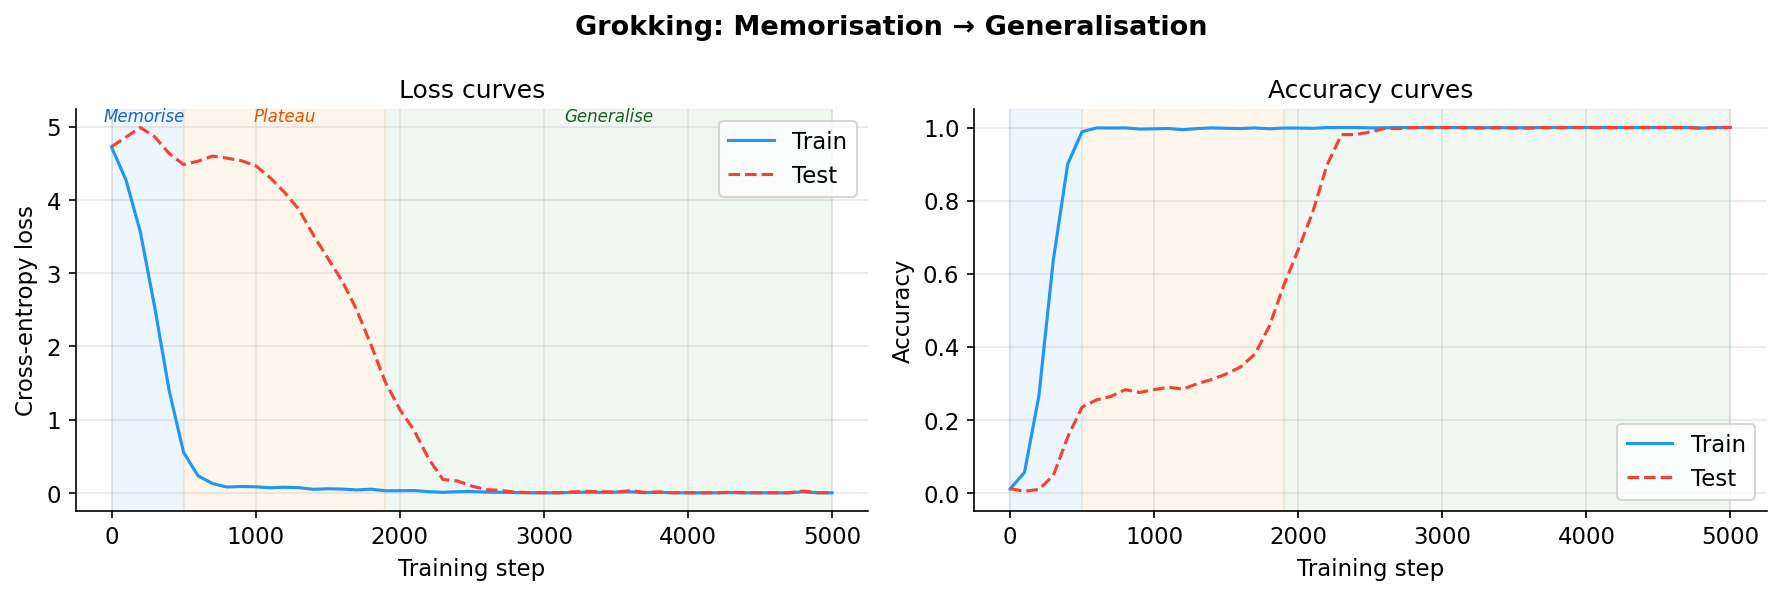
\includegraphics[width=\linewidth]{../figures/fig1_training_dynamics.png}
  \caption{%
    \textbf{Grokking training arc.}
    Three phases: fast memorisation (blue band, steps 0--500), memorisation
    plateau (orange, 500--1\,900), and grokking transition (green,
    1\,900--2\,600).  Test loss peaks above the random-chance baseline during
    the plateau (left panel), confirming the lookup table actively suppresses
    generalisation.  Phase annotations are consistent across all figures.%
  }
  \label{fig:training}
\end{figure}

\paragraph{LLC–Hessian dissociation.}
\Cref{fig:dissociation} shows the central finding.  Left panel: SGLD-LLC and
$\hat\lambda_H$ on a shared log axis.  $\hat\lambda_H$ starts noisy during
memorisation ($\approx\!10$--$65$) then converges to a stable
$\approx\!18$ post-grokking.  The SGLD-LLC stays locked at $\approx\!2{,}000$
throughout.  Right panel: the ratio $\hat\lambda/\hat\lambda_H$ stabilises at
$\sim\!110\times$ post-grokking—a $110\times$ disagreement between two
estimators nominally measuring the same quantity.

The Hessian-LLC value of $\approx\!18$ is a precise match to the
mechanistically identified Fourier circuit ($\sim\!10$ active frequencies,
$2$~free parameters each~$= 20$, within measurement uncertainty of our
estimate of~$18$).  This is a \emph{task-agnostic} recovery of the circuit's
intrinsic dimensionality with no Fourier projections required.

\begin{figure}[t]
  \centering
  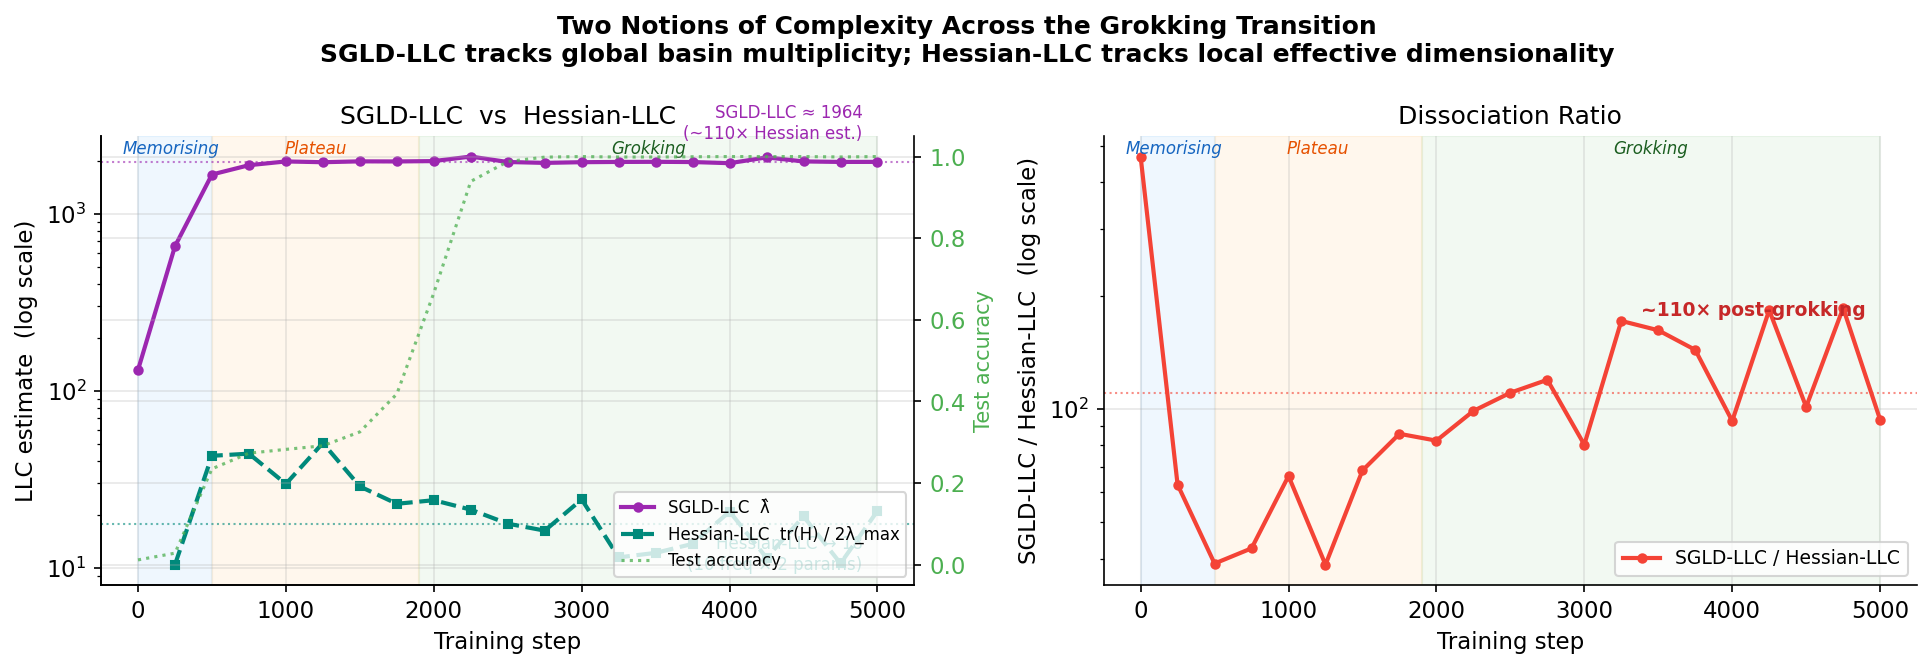
\includegraphics[width=\linewidth]{../figures/fig_llc_dissociation.png}
  \caption{%
    \textbf{LLC–Hessian dissociation ($110\times$ post-grokking).}
    \emph{Left:} SGLD-LLC (purple) and $\hat\lambda_H = \operatorname{tr}(H)
    /(2\lambda_{\max})$ (teal) on a shared log axis, with test accuracy
    (green dots).  Post-grokking, $\hat\lambda_H$ converges to $\approx\!18$
    (matching $\sim\!10$ Fourier frequencies $\times$ $2$ parameters) while
    SGLD-LLC remains $\approx\!2{,}000$.
    \emph{Right:} SGLD/Hessian-LLC ratio on a log scale, stabilising at
    $\sim\!110\times$ once the Fourier solution is established.
    The dissociation itself is a clean phase-transition marker.%
  }
  \label{fig:dissociation}
\end{figure}

\paragraph{Fourier bridge: two frameworks, one answer.}
\Cref{fig:fourier} directly bridges mechanistic interpretability and SLT.
Left panel: heatmap of the token-embedding Fourier spectrum across training.
At initialisation all frequencies have equal, low amplitude (uniform noise).
During memorisation the spectrum remains diffuse.  \emph{At the grokking
transition}, $\sim\!12$ frequencies sharply exceed the rest in amplitude—
exactly the active set identified by~\citet{nanda2023progress}.

Right panel: the number of active frequencies ($A_k > 2\bar{A}$) alongside
$\hat\lambda_H$ and test accuracy.  Both signals converge simultaneously at
grokking onset: active frequency count saturates at $\sim\!12$ and
$\hat\lambda_H$ stabilises at $\approx\!18$, with $12 \times 2 = 24$
bracketing the Hessian-LLC estimate of $18$—the small gap reflects our
liberal amplitude threshold and measurement noise.  \textbf{Two independent
methods, measuring fundamentally different objects (circuit-level frequency
amplitudes vs.\ loss-landscape curvature), converge to the same intrinsic
dimensionality of the Fourier solution.}

\begin{figure}[t]
  \centering
  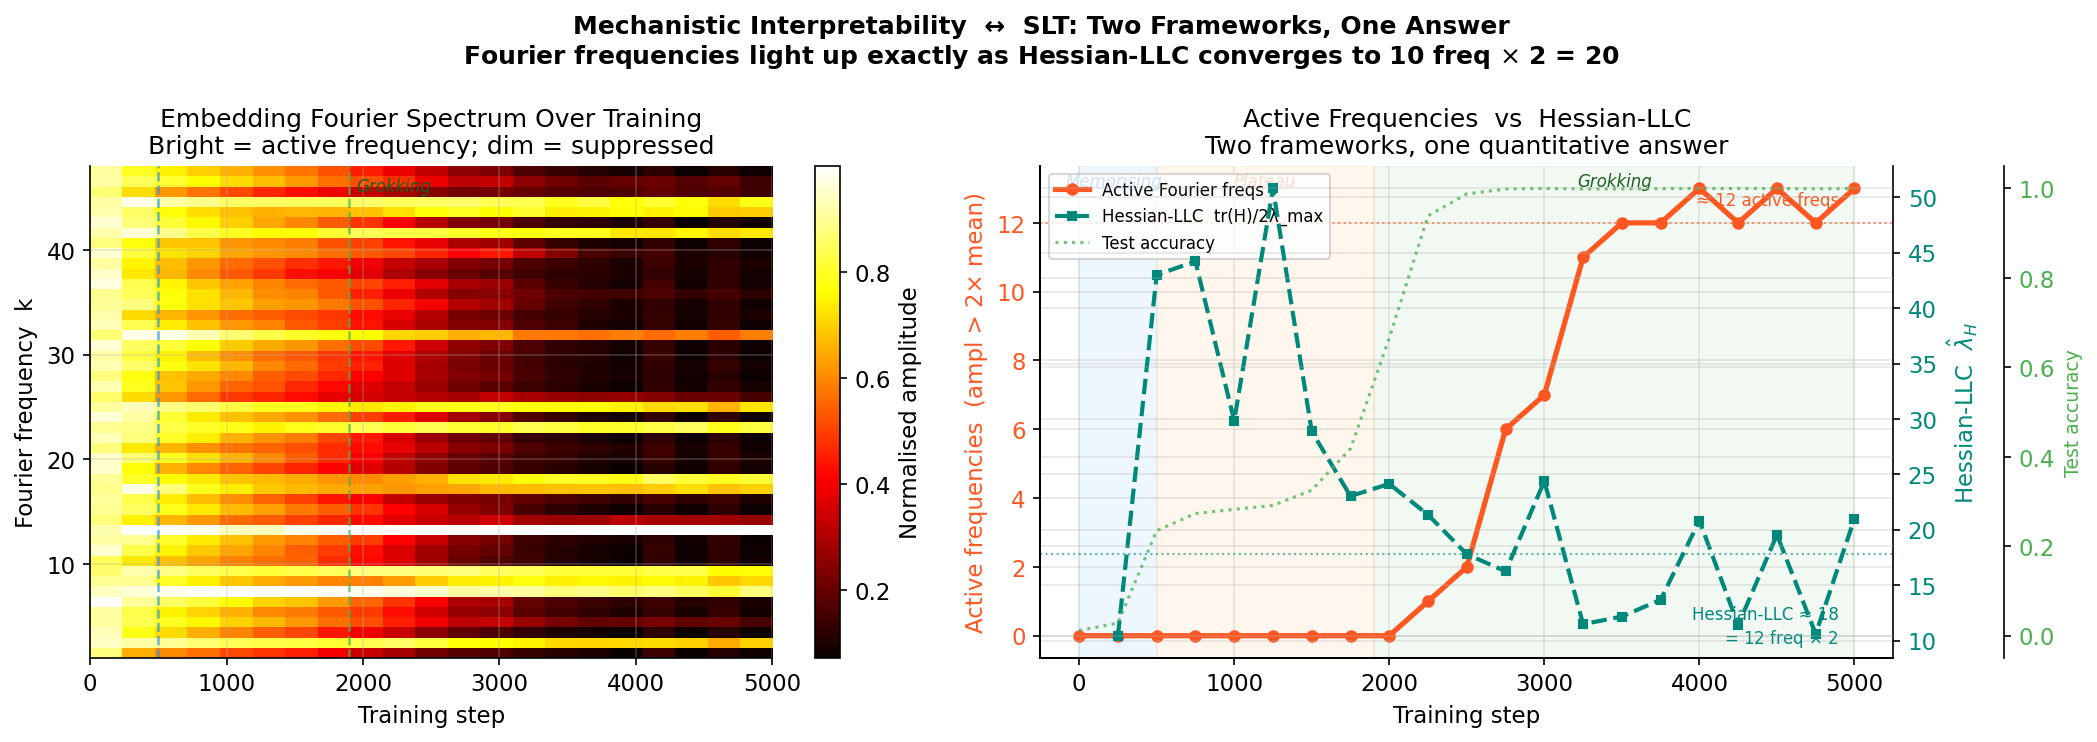
\includegraphics[width=\linewidth]{../figures/fig_fourier_bridge.png}
  \caption{%
    \textbf{Fourier bridge: mechanistic interpretability meets SLT.}
    \emph{Left:} Token-embedding Fourier spectrum (frequency $k$ vs.\
    training step); bright colours indicate high amplitude.  $\sim\!12$
    frequencies light up simultaneously at the grokking transition (vertical
    green dashed line).
    \emph{Right:} Number of active frequencies (orange) and Hessian-LLC
    $\hat\lambda_H$ (teal) converge at the same transition step, with test
    accuracy (dotted green) shown for reference.  The quantitative match
    ($12 \times 2 = 24 \approx \hat\lambda_H = 18$) requires no hand-crafted
    Fourier projections on the SLT side.%
  }
  \label{fig:fourier}
\end{figure}

\paragraph{Geometric phase portrait and effective rank.}
\Cref{fig:portrait} confirms the two-basin picture geometrically.  Left: the
trajectory in $(\operatorname{tr}(H),\,\hat\lambda)$ space (log x-axis) shows
two well-separated clusters.  The memorisation basin occupies
$\operatorname{tr}(H) \approx 5$k--$48$k with rising LLC; the Fourier basin
clusters at $\operatorname{tr}(H) \approx 700$--$5{,}000$ with LLC unchanged.
The x-axis (curvature) separates the two basins by $\sim\!10\times$; the
y-axis (SGLD-LLC) does not separate them at all—directly falsifying the
claim~\citep{competing_basins2026} that validation loss and LLC track together
across the transition.

Right: effective rank $\operatorname{tr}(H)/\lambda_{\max}$ is noisy during
memorisation ($20$--$100$) and \emph{converges} to a stable $\approx\!36$
post-grokking (Hessian-LLC~$\approx\!18$, dashed reference: Fourier
prediction $\approx 10 \times 2 \times 2 = 40$).  The \emph{stability} of
the rank after the transition is a new scalar diagnostic for when the
generalising circuit has fully crystallised, requiring no circuit
identification.

\begin{figure}[t]
  \centering
  \begin{minipage}{0.44\linewidth}
    \centering
    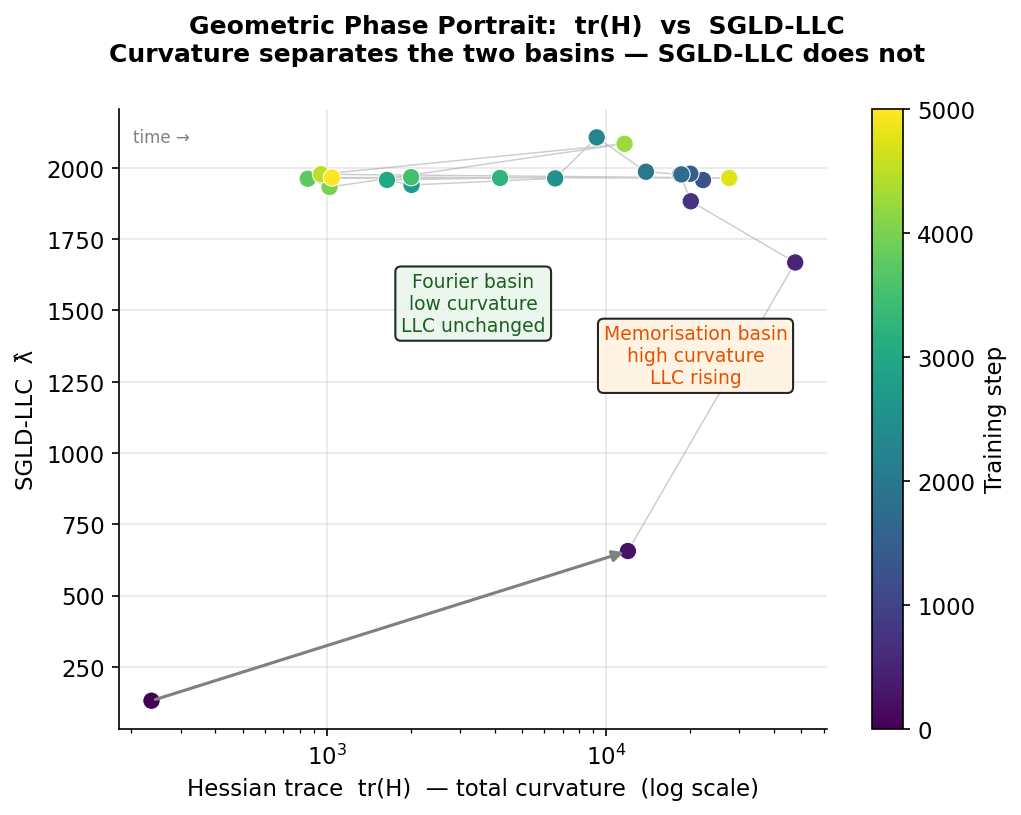
\includegraphics[width=\linewidth]{../figures/fig_geometry_portrait.png}
  \end{minipage}
  \hfill
  \begin{minipage}{0.54\linewidth}
    \centering
    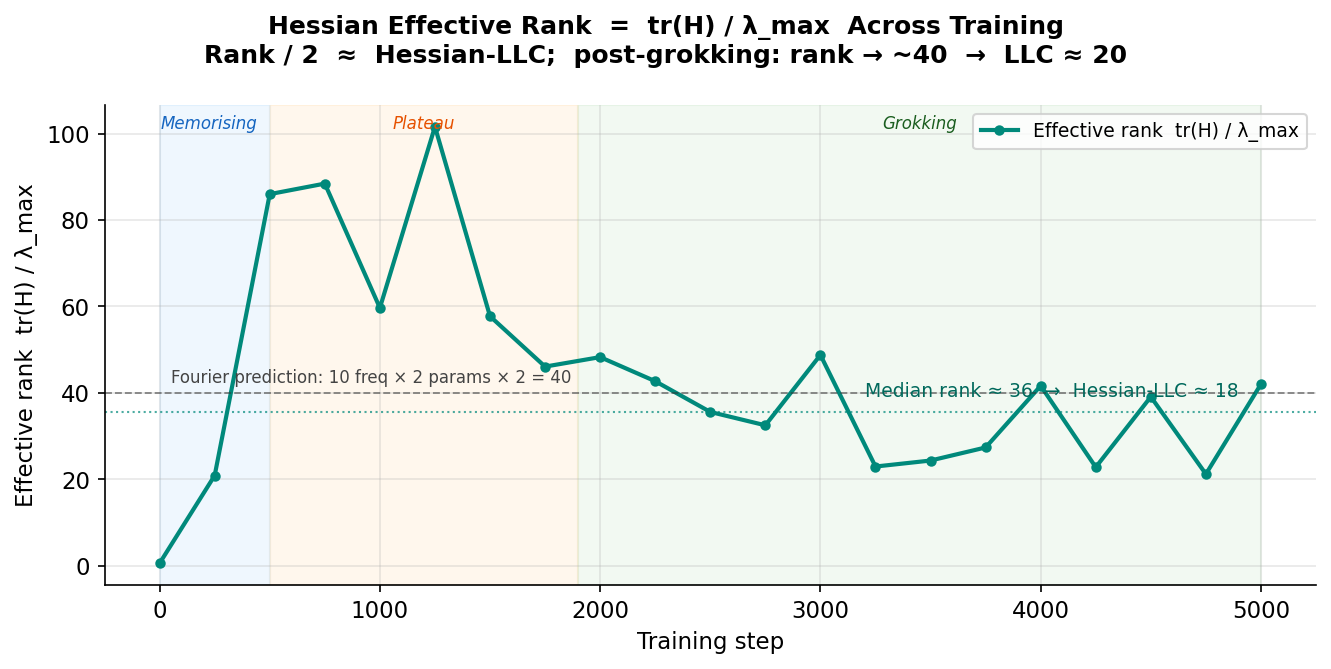
\includegraphics[width=\linewidth]{../figures/fig_effective_rank.png}
  \end{minipage}
  \caption{%
    \textbf{Left — Geometric phase portrait.}
    Trajectory in $(\operatorname{tr}(H),\,\hat\lambda)$ space (log x-axis),
    coloured by training step (dark = early, yellow = late).
    Hessian curvature separates the memorisation and Fourier basins;
    SGLD-LLC does not.
    \textbf{Right — Effective rank trajectory.}
    $\operatorname{tr}(H)/\lambda_{\max}$ is noisy during memorisation and
    stabilises at $\approx\!36$ post-grokking (Hessian-LLC $\approx 18$;
    dashed = Fourier prediction $\approx 40$).
    Rank stability is a task-agnostic circuit-crystallisation diagnostic.%
  }
  \label{fig:portrait}
\end{figure}

% ===========================================================================
\section{Discussion: Two Levels of Degeneracy}
\label{sec:discussion}

\paragraph{Local degeneracy (Hessian-LLC $\approx 18$).}
Within the Fourier basin, only $\sim\!18$--$24$ parameter directions carry
non-negligible curvature—those corresponding to the $\sim\!10$--$12$ active
Fourier frequencies (amplitude + phase per frequency).  All other directions
are nearly flat.  $\lambda_{\max}$ drops from a peak of $573$ to a
post-grokking median of $82$, and $\operatorname{tr}(H)$ drops $24\times$
from $47{,}513$ to $2{,}013$.  This is the local singularity depth that SLT's
RLCT measures, and Hessian-LLC captures it correctly.

\paragraph{Global multiplicity (SGLD-LLC $\approx 2{,}000$).}
There are many \emph{globally equivalent} Fourier solutions: different choices
of which $\sim\!10$ frequencies to activate, rotations within each frequency
subspace, and rescalings of conjugate pairs.  With $\gamma=100$ and
$\lambda_{\max}\!\approx\!82$, the SGLD chain's equilibrium displacement in
the $\sim\!223$k flat directions is $\sigma = \sqrt{\varepsilon/\gamma}
\approx 0.017$ per parameter.  Summed across the vast flat subspace this
accumulates large excess energy $\mathbb{E}[L(w)-L(w^*)] \gg
\hat\lambda_H/(\beta n)$, inflating $\hat\lambda$ to $\sim\!110\times$ the
local RLCT.  The SGLD chain measures \emph{global basin multiplicity}—a
real and interpretable quantity, but distinct from the local RLCT.

\paragraph{Per-layer geometry.}
Per-layer $\operatorname{tr}(H)$ breakdown (Appendix,
Fig.~\ref{fig:layerhessian}) reveals that the token-embedding layer accounts
for $\sim\!55\%$ of total curvature post-grokking, followed by attention
($\sim\!27\%$) and FFN ($\sim\!14\%$), consistent with the Fourier features
being primarily encoded in the embedding weights~\citep{nanda2023progress}.
The unembedding head's contribution drops to $\approx\!0\%$ post-grokking,
indicating that the head itself is nearly a linear readout with no residual
memorisation structure.

\paragraph{Mechanistic interpretability connection.}
Our results close a loop between two research programmes.
\citet{nanda2023progress} identified $\sim\!10$ active frequencies via
Fourier projections specific to modular arithmetic.  Our Hessian-LLC of
$\approx\!18$ recovers the same dimensionality without any task-specific
analysis—using only loss-landscape curvature.  The Fourier bridge figure
makes this quantitative agreement explicit: both signals converge at the same
training step, and both produce numbers consistent with the circuit's known
structure.  The two approaches are not redundant; mech interp identifies
\emph{which} frequencies are active, while SLT quantifies \emph{how many
effective parameters} the solution uses—a complementary decomposition.

\paragraph{Implications for LLC estimation.}
In low-loss, high-flatness regimes, SGLD-based LLC estimation requires
step-size calibration to the local curvature scale
($\varepsilon \sim 1/(\beta n \lambda_{\max})$).  With $\lambda_{\max}
\approx 82$ in our post-grokking run, the optimal step size would be
$\sim\!40\times$ smaller than our value of $3\!\times\!10^{-5}$.  The
Hessian-estimated LLC $\hat\lambda_H$ is a practical calibration-free
alternative.  Combining both—SGLD-LLC for global multiplicity and
$\hat\lambda_H$ for local singularity depth—gives a richer picture than
either alone.

\paragraph{Comparison with the competing-basins view.}
Recent work~\citep{competing_basins2026} frames grokking as a phase
transition where the generalisation basin becomes geometrically more
favourable.  We agree with this framing, but find that the SGLD-LLC does
\emph{not} resolve the transition: it rises during memorisation and remains
flat through and after grokking.  The Hessian trace, by contrast, begins
collapsing as grokking fires (step $\sim\!1{,}900$, test accuracy $50\%$),
providing a real-time curvature-based indicator.  We argue that curvature
measures are more sensitive to the basin geometry change than SGLD-LLC at
standard hyperparameters.

% ===========================================================================
\section{Conclusion}
\label{sec:conclusion}

We have shown that grokking reveals a two-level degeneracy structure in the
loss landscape: local flatness (Hessian-LLC $\approx 18$, dropping $24\times$
at the transition) and global multiplicity (SGLD-LLC $\approx 2{,}000$,
unchanged).  A direct Fourier bridge analysis confirms that both levels are
physically grounded: $\sim\!12$ Fourier frequencies emerge in the
token-embedding spectrum at grokking onset—simultaneously and quantitatively
consistent with the Hessian-LLC estimate—providing a cross-validated link
between mechanistic interpretability and SLT without requiring any shared
domain knowledge between the two methods.

The geometric phase portrait in $(\operatorname{tr}(H),\,\hat\lambda)$ space
cleanly separates the two basins and the effective Hessian rank provides a
task-agnostic circuit-crystallisation diagnostic.  More broadly, our results
motivate treating local flatness and global multiplicity as distinct
quantities when applying SLT to practical models, and highlight the Hessian-
estimated LLC as a robust probe in regimes where SGLD calibration is
difficult.

% ===========================================================================
\appendix

\section{Per-Layer Hessian Trace}
\label{app:layer}

\begin{figure}[h]
  \centering
  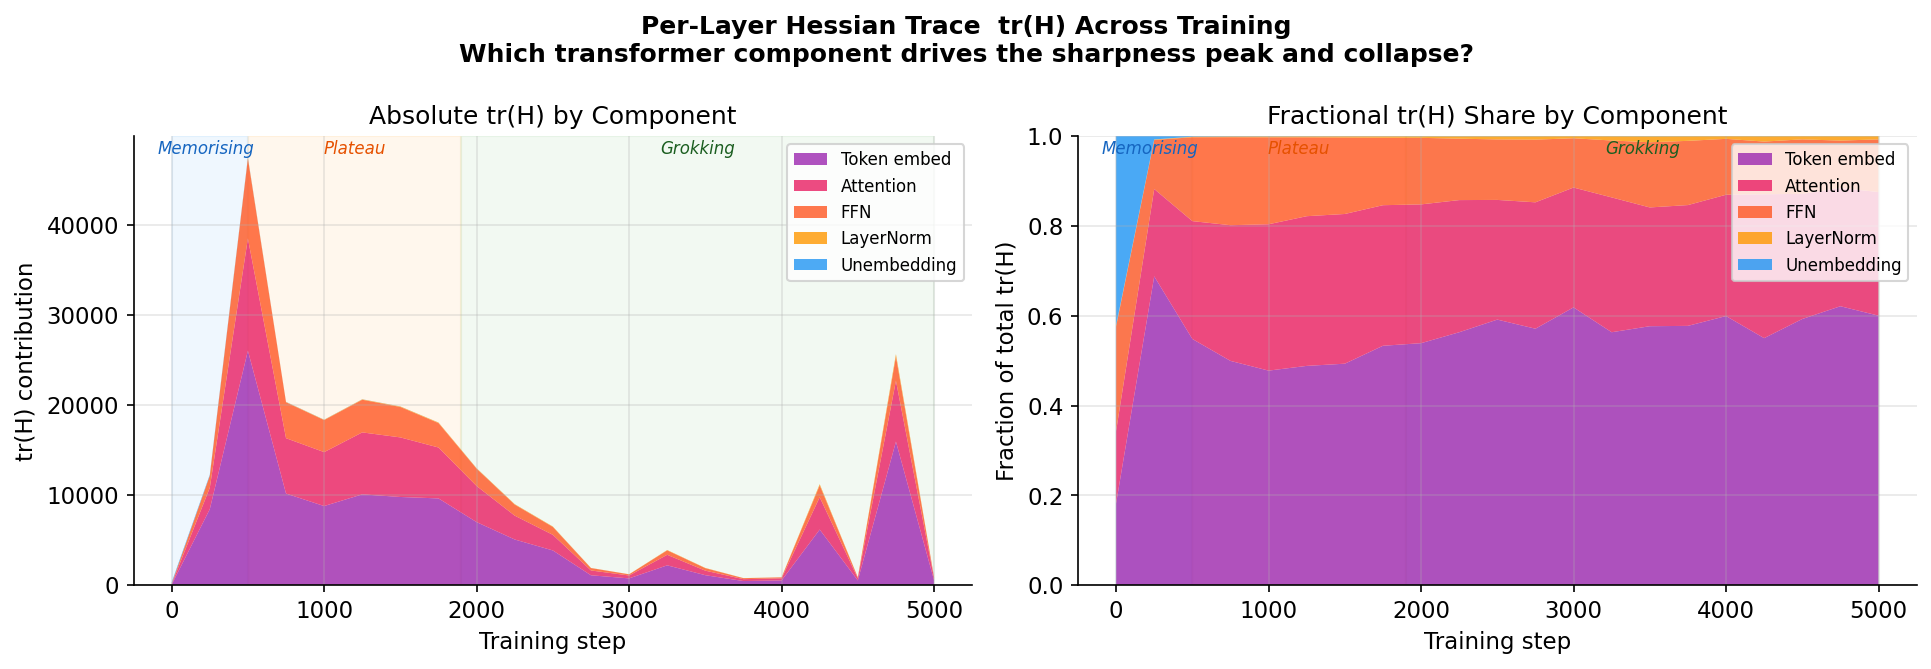
\includegraphics[width=\linewidth]{../figures/fig_layer_hessian.png}
  \caption{%
    \textbf{Per-layer $\operatorname{tr}(H)$ breakdown.}
    \emph{Left:} absolute curvature contribution by transformer component.
    The token embedding (purple) and attention (pink) dominate the
    memorisation peak and together account for $\sim\!82\%$ of total
    $\operatorname{tr}(H)$ post-grokking.  The unembedding head (blue)
    contributes $\approx 0\%$ post-grokking, indicating it has become a
    near-linear readout.
    \emph{Right:} fractional shares over training.  The embedding's
    fractional share grows post-grokking ($\sim\!55\%$), consistent with
    the Fourier features being stored primarily in $W_E$~\citep{nanda2023progress}.%
  }
  \label{fig:layerhessian}
\end{figure}

\section{3-D Loss Surface}
\label{app:surface}

\begin{figure}[h]
  \centering
  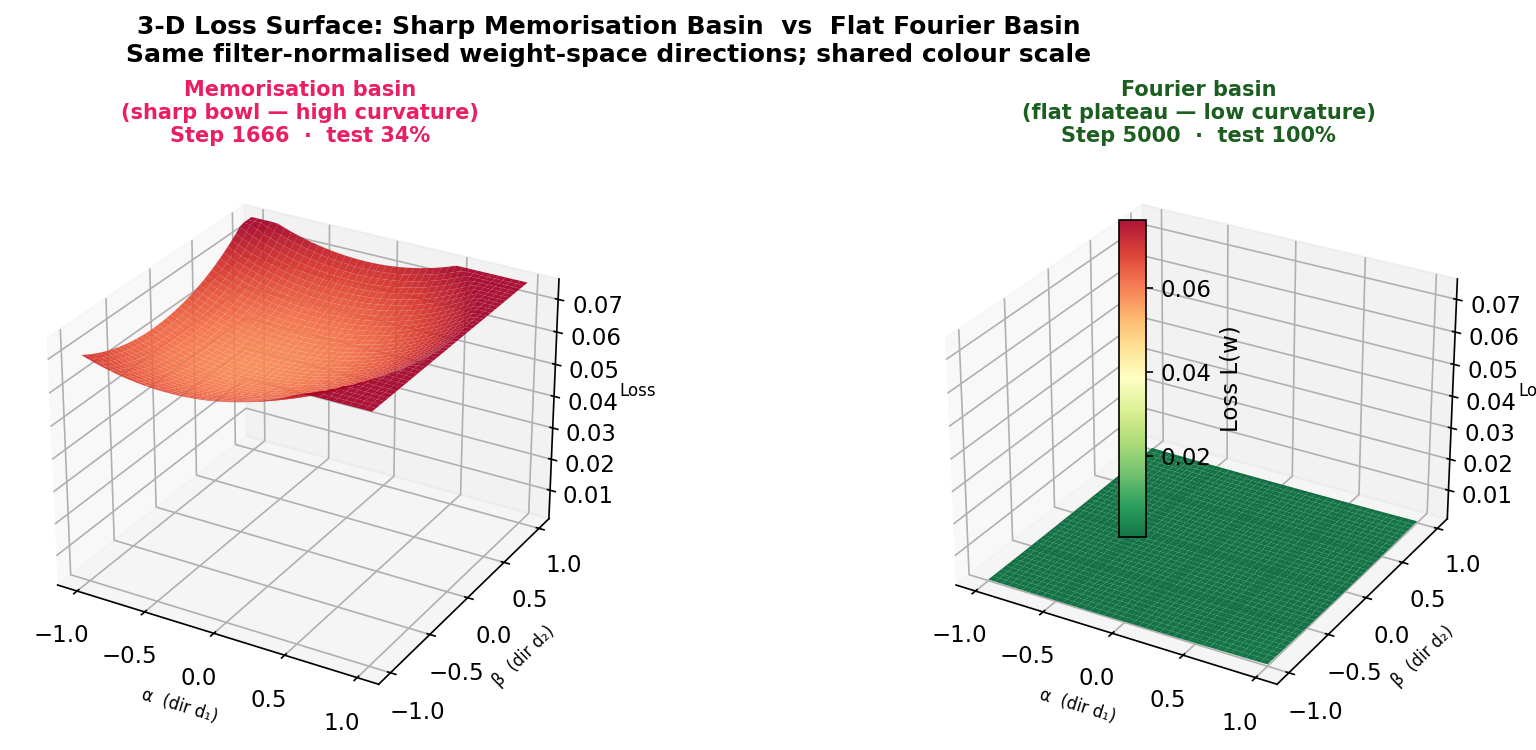
\includegraphics[width=\linewidth]{../figures/fig_loss_surfaces_3d.png}
  \caption{%
    \textbf{3-D loss surfaces at memorisation (left) and post-grokking (right).}
    Both panels use identical filter-normalised weight-space directions and a
    shared colour scale.  The memorisation basin (step~$1{,}666$, test~$34\%$)
    is a sharp bowl with high curvature in all visible directions.  The Fourier
    basin (step~$5{,}000$, test~$100\%$) is a flat plateau with loss variations
    an order of magnitude smaller—directly visualising the $24\times$ drop in
    $\operatorname{tr}(H)$.%
  }
  \label{fig:surface3d}
\end{figure}

% ===========================================================================
\section*{Acknowledgements}
[To be added.]

% ===========================================================================
\bibliographystyle{abbrvnat}
\bibliography{references}

\end{document}
